\documentclass[12pt, a4]{article}
\usepackage[english]{babel}
\usepackage[utf8x]{inputenc}
\usepackage{fullpage}
\usepackage{listings}
\usepackage{graphicx}
\usepackage{color}

%Syntax highlighting
\definecolor{blue-violet}{rgb}{0.54, 0.17, 0.89}
\definecolor{ao}{rgb}{0.0, 0.5, 0.0}
\definecolor{amaranth}{rgb}{0.9, 0.17, 0.31}
\definecolor{ballblue}{rgb}{0.13, 0.67, 0.8}
\definecolor{onyx}{rgb}{0.06, 0.06, 0.06}


\lstset{
  breaklines=true,                 % automatic line breaking only at whitespace
  captionpos=b,                    % sets the caption-position to bottom
  breakatwhitespace=false,
  keepspaces=true,
  numbers=left,
  numbersep=5pt,
  showspaces=false,
  showstringspaces=false,
  showtabs=false,
  tabsize=4,  
  backgroundcolor=\color{white},   % choose the background color
  commentstyle=\color{ao},    % comment style
  keywordstyle=\color{amaranth},    % keyword style
  stringstyle=\color{blue-violet},    % string literal style
  numberstyle=\tiny\color{ballblue},	   % number style
  basicstyle=\ttfamily\footnotesize\color{onyx} % size of fonts used for the code
}

%Document Header
\title{\textbf{Department of CSE\\SSN College of Engineering}}
\author{\textbf{Vishakan Subramanian - 18 5001 196 - Semester VII}}
\date{19 July 2021}

\begin{document}
\maketitle
\hrule
\section*{\center{UCS 1712 - Graphics And Multimedia Lab}}
\hrule
\bigskip

%Assignment Details
\subsection*{\center{\textbf{Exercise 1: Study of Basic Output Primitives in C++ using OpenGL}}}
\subsection*{\flushleft{Aim:}}
\begin{flushleft}
\begin{itemize}
\item To create an output window using OPENGL and to draw the following basic output primitives - POINTS, LINES, LINE STRIP, LINE LOOP, TRIANGLES, QUADS, QUAD STRIP, POLYGON.
\item To create an output window and draw a checkerboard using OpenGL. 
\item To create an output window and draw a house using POINTS, LINES, TRIANGLES and QUADS/POLYGON.  

\end{itemize}
\end{flushleft}

%Code
\newpage
\subsection*{\flushleft{Code: Basic Primitives:}}
\begin{flushleft}
\lstinputlisting[language = C]{Primitives/main.cpp}
\end{flushleft}

%Code
\newpage
\subsection*{\flushleft{Code: Checker Board}}
\begin{flushleft}
\lstinputlisting[language = C]{Checkerboard/main.cpp}
\end{flushleft}

%Code
\newpage
\subsection*{\flushleft{Code: House}}
\begin{flushleft}
\lstinputlisting[language = C]{House/main.cpp}
\end{flushleft}


%Output
\newpage
\subsection*{\flushleft{Output: Primitives:}}
\begin{figure}[h]
\centering
\caption{Output: Primitives.}
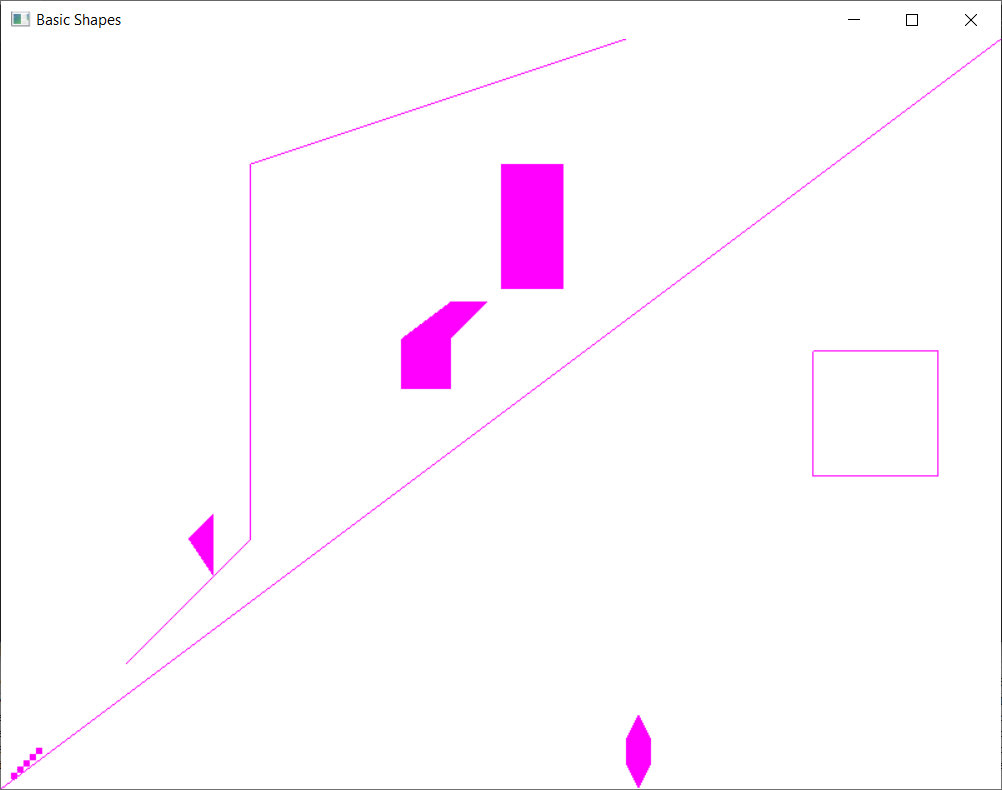
\includegraphics[height=11.25cm, width=15cm]{Primitives/Output.png}
\end{figure}

%Output
\newpage
\subsection*{\flushleft{Output: Checker Board:}}
\begin{figure}[h]
\centering
\caption{Output: Checker Board.}
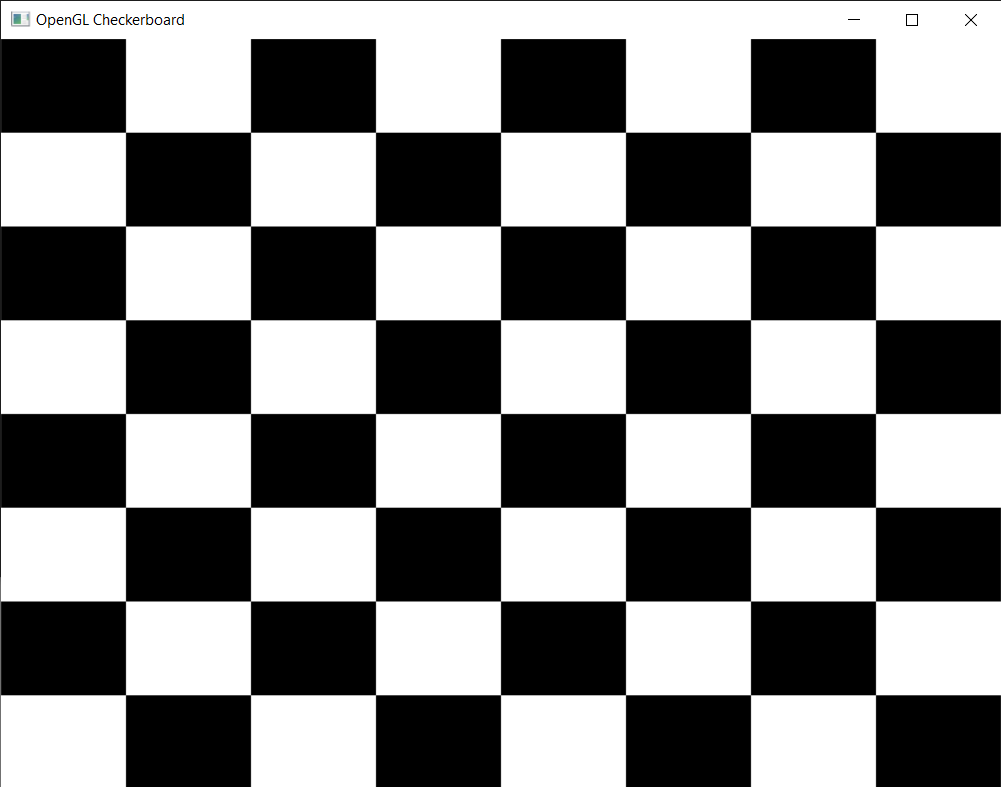
\includegraphics[height=11.25cm, width=15cm]{Checkerboard/Output.png}
\end{figure}

%Output
\newpage
\subsection*{\flushleft{Output: House:}}
\begin{figure}[h]
\centering
\caption{Output: House.}
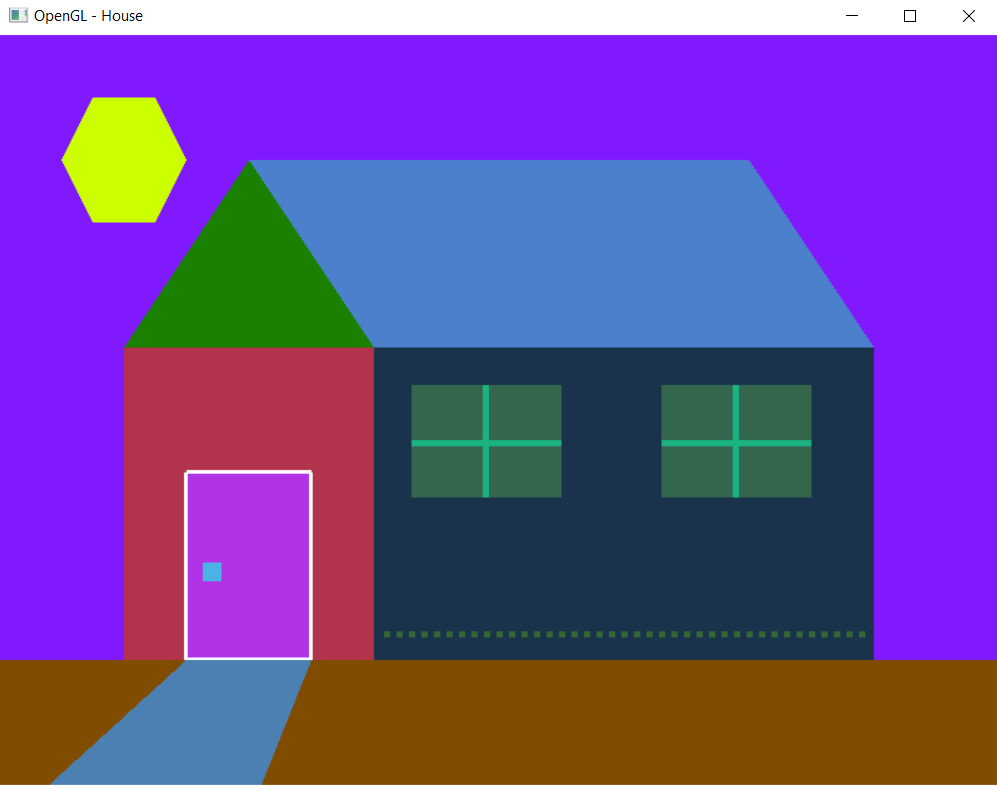
\includegraphics[height=11.25cm, width=15cm]{House/Output.png}
\end{figure}

%Learning Outcome
\newpage
\subsection*{\flushleft{Learning Outcome:}}
\begin{itemize}
\item I configured \textbf{OpenGL} and \textbf{GLUT Framework} on my system using the CodeBlocks IDE.
\item I learnt about OpenGL and its usage in the high-performance graphics industry - like creating animations and games.
\item I learnt to draw some \textbf{primitive output shapes} like points, lines, line strips, line loops, triangles, quads, quad strips and polygons using GLUT's inbuilt functions.
\item I understood how to \textbf{initialize a new GLUT output display} with colors, matrix mode, window title, window size etc.
\item I learnt how these shapes are plotted using the \textbf{glVertex2d()} function.
\item I was able to construct a basic \textbf{8x8 checkerboard} using the inbuilt primitive functions and was able to color the checkerboard appropriately.
\item I was able to draw a \textbf{simple house} with shapes like triangles, quads and polygons. I was also able to color the house with different shades.
\item I understood that the OpenGL uses a \textbf{coordinate system} to map the output shapes onto the display window. 

\end{itemize}


\end{document}